\chapter{System Architecture}

\section{Overview}

\begin{figure}[h]
  \centering
  \pgfdeclarelayer{background}
\pgfdeclarelayer{foreground}
\pgfsetlayers{background,main,foreground}

\begin{tikzpicture}
  \node[](management){\pgfdeclarelayer{background}
\begin{tikzpicture}
  \node[](key-comp){\begin{tikzpicture}
  % Define distances for bordering
  \def\blockdist{2.3}
  \def\edgedist{2.5}

  % Draw components
  \node[component](status-checker){Status Checker};
  \path (status-checker.south)+(0,-4.2) node[component](decision-maker){Decision Maker};
  \path (status-checker.north east)+(\blockdist,0) node[dispatcher, anchor=north west](dispatcher){Dispatcher};
  \draw[vecArrow] ([xshift=-10]status-checker.south) to ([xshift=-10]decision-maker.north);
  \draw[vecArrow] ([xshift=10]decision-maker.north) to ([xshift=10]status-checker.south);

  % Draw interaction arrows
  \def\composhift{50}
  \draw[vecArrow] ([yshift=-10]status-checker.east) to ([yshift=-10+\composhift]dispatcher.west);
  \draw[vecArrow] ([yshift=10+\composhift]dispatcher.west) to([yshift=10]status-checker.east);

  \draw[vecArrow] ([yshift=-10]decision-maker.east) to ([yshift=-10-\composhift]dispatcher.west);
  \draw[vecArrow] ([yshift=10-\composhift]dispatcher.west) to ([yshift=10]decision-maker.east) ;
\end{tikzpicture}
};
  \path (key-comp.south) + (0, -0.5) node(comp-caption){Management System};
  \begin{pgfonlayer}{background}
    \node[system,fit=(key-comp) (comp-caption)]{} ;
  \end{pgfonlayer}
\end{tikzpicture}
};

  % Client
  %\coordinate (client-mid) at (management.east) + (5em,0);
  %\path (client-mid) + (0,-2) node[component,text width=5em]{Client};
  %\path (client-mid) + (0, 2) node[component,text width=5em]{Client};

  % Workers
  \coordinate (l1) at (management.south west);
  \coordinate (l2) at (management.south east);
  \path (l1) + (0, -3)
  node[component,text width=4em,minimum height=3em](w1){worker};
  \path (l2) + (0, -3)
  node[component,text width=4em,minimum height=3em](w4){worker};
  \path ($(w1)!0.33!(w4)$)
  node[component,text width=4em,minimum height=3em](w2){worker};
  \path ($(w1)!0.66!(w4)$)
  node[component,text width=4em,minimum height=3em](w3){worker};
  \draw[vecArrow] ([xshift=-5]$(l1)!0.2!(l2)$) to ([xshift=-5,yshift=3]w1.north);
  \draw[vecArrow] ([xshift=-5]$(l1)!0.4!(l2)$) to ([xshift=-5,yshift=3]w2.north);
  \draw[vecArrow] ([xshift=-5]$(l1)!0.6!(l2)$) to ([xshift=-5,yshift=3]w3.north);
  \draw[vecArrow] ([xshift=-5]$(l1)!0.8!(l2)$) to ([xshift=-5,yshift=3]w4.north);
  \draw[vecArrow] ([xshift=5,yshift=3]w1.north) to ([xshift=5]$(l1)!0.2!(l2)$);
  \draw[vecArrow] ([xshift=5,yshift=3]w2.north) to ([xshift=5]$(l1)!0.4!(l2)$);
  \draw[vecArrow] ([xshift=5,yshift=3]w3.north) to ([xshift=5]$(l1)!0.6!(l2)$);
  \draw[vecArrow] ([xshift=5,yshift=3]w4.north) to ([xshift=5]$(l1)!0.8!(l2)$);
\end{tikzpicture}


  \caption{System Architecture Overview}
  \label{fig:archi-overview}
\end{figure}

%%% begins with introducing the system and what is does again as a reminding
We proposed a cloud resource management framework to dynamically adjust
the number of physical servers for a single job.
The framework make decisions according to some specified policies.
The policies take the remaining workload, priority and deadline of each
job into consideration, and generate a scheduling plan that satisfies
the job requirements.
%%%
This framework can work as an individual cloud computing system, or as
extension components of an existent cloud system.

% Overview
Figure~\ref{fig:archi-overview} shows the architecture of our cloud
management framework.
The core part is the management system, which consists of three
components: \emph{status checker}, \emph{decision maker} and
\emph{dispatcher}.
%%% move this sentence to the previous paragraph
%The whole framework can form a complete cloud computing system or work
%as a part of existent cloud systems.

%%% TODO change this sentence into work flows, how worker and client interactive with our system
% TODO use the topic sentence of each component to briefly describe it.
In the former case, the management system connects with several
\emph{workers}, which leverage physical resources directly, and
interacts with instances of \emph{client} --- the interface end users
submit jobs from.

% RPC server design
We implemented the management components and the worker as separate RPC
(remote procedural call)~\cite{cite:RPC} servers.
Separate RPC server implementation makes each component
\emph{pluggable}.
The pluggability gives the system administrator flexibility to choose
the most suitable component implementation to fit different needs.
Moreover, without shutting the whole system down, it is possible to
change system configurations --- or even upgrade the system --- by
substituting target components with feasible ones.
Besides, this design allows us to easily integrate the management system
with other cluster management frameworks like JPPF~\cite{cite:JPPF} or
cloud operating system like Roystonea~\cite{cite:roystonea}.
Roystonea~\cite{cite:roystonea} also benefits from the RPC server
implementation.

%%% Not sure if we need this, but anyway...
The rest of the chapter is organized as followed.  
First we introduce the \emph{client}, which is ...
Then we define the \emph{Worker} in our system, ...
The three components, { \emph{status checker}, \emph{decision maker} and
\emph{dispatcher}, are described after that.

\section{Job and Tasks}

Before discussing our system architecture, we have to introduce the
representation of workload in our system.
Users will submit \emph{jobs} each of which consists of several
\emph{tasks}, the minimum unit of scheduling, to the system.
As a cluster management framework, submitted jobs are meant to be
expected to be processed in parallel.
It is end user's responsibility to split their jobs into balanced tasks.
Just like all of other parallel computing systems, the more balanced the
tasks, the better the system schedules.

\section{Client}

% Client is the interface of submission
The client is the programming interface for users to submit jobs to our
system.
In our framework, a user will submit \emph{jobs} to the system via a
client instance created using the provided library.

% attributes
Users specify several attributes to jobs before submission, such as
deadline, priority and execution profile from previous experience.
These attributes are later passed to decision maker for reference so
that it can schedule the jobs.

% Library features: batch submission and background execution
The client library also provides several features to end users to
satisfy their varying programming needs.
First, we support background task execution, which means users can
specify the synchronization point that waits all the submitted task to
be done as they like, without blocking the code before it.
Besides, user can submit multiple jobs at a time.
Combining these two features, user can easily program the
synchronization model they want, just like those traditional work flow
description languages can do~\cite{cite:workflow-management}.
Here's an example on how to program with our client library.

% Programming example
\newfloat{Example Code}{H}{myc}
\lstloadlanguages{Ruby}
\begin{Example Code}
  \begin{lstlisting}[language=Ruby]
  client = Client.new
  client.register(SERVER_ADDRESS)
  client.start
  j1 = Job.new('Job1')
  j1.add_task Task.new(...)
  ... # Add more tasks
  j2 = Job.new('Job2')
  j2.add_task Task.new(...)
  ... # Add more tasks
  # 200-second deadline
  j1.deadline = j2.deadline = Time.now + 200.0
  # Submit j1 and j2 together
  # Background execution
  j12_waiter = client.submit_job([j1,j2])
  # Do other time consuming computation
  ...
  j3 = Job.new('Job3')
  j3.add_task Task.new(...)
  ... # Add more tasks
  # Remaining part can't run until j3 is done
  j3_waiter = client.submit_job(j3)
  client.wait(j3_waiter)
  # Some more things to do
  ...
  # Wait until j1 and j2 is done.
  client.wait(j12_waiter)
  # Combning j1, j2 and j3
  ...
\end{lstlisting}

  \caption{Sample code of client usage}
\end{Example Code}

Assume that the user has 3 jobs --- $j_1$, $j_2$ and $j_3$ --- to be
done separately and their result to be aggregated:  $j_1$ and $j_2$
takes long time to run on the cluster can be submitted directly; $j_3$
takes shorter time on remote clusters if separated into parallel tasks
but requires time consuming local pre-processing and post-processing.
Since $j_1$, $j_2$ and pre-processing of $j_3$ is costive, it's better
to do them in parallel.
As a result, we submit $j_1$ and $j_2$ at first and wait for their
results in the background then start pre-processing $j_3$. Not needing
post-processing, results of $j_1$ and $j_2$ are synchronized after
$j_3$.
Finally, as all of the results come back, we can do the final
aggregation.

\section{Worker}

Workers are the ones using resource of the cloud directly.
They execute tasks assigned by the management system.
A worker instance executes at most one task at a time, but it doesn't
mean that a physical machine can run one task only at a time.
One can run multiple worker instances on a physical machine so that a
physical machine could run more than one task simultaneously.	 

Deploying multiple worker instances on a powerful machine (e.g., with
large number of cores) can gain better performance from
multiprogramming, but in contrary, it might however cause resource
contention on low-end machines.
We leave the choice to system administrators.


If the task execution performance of a machine running multiple worker
instances is far worse than expected, it is very likely due to resource
contention.
In that case, the system administrator should consider reducing the
number of worker instances on that machine.
Thanks to the pluggable implementation, this can be done \emph{online},
without stopping any of other components, even running workers which is
preferred to keep on that machine, by simply stop several worker
instances.

% TODO  Should I move this to another section???
In fact, our management system can function without workers.
In the case that it is working as a part of other cluster management
frameworks, the framework in charge should be responsible for
manipulating physical resources instead.

\section{Status Checker}

Status checker periodically collects the information about worker
instances and physical servers.
Leveraging the information collected by status checker, the decision
maker can make resource allocation plans according to a policy specified
by the system administration.

The most essential information for the system is probably the status of
workers.
A worker can be in status of either \emph{available}, \emph{occupied},
\emph{busy} or \emph{down}.
Available means the worker
is idle and ready to accept task assignment; occupied indicates that the
worker is assigned to a job but executing any task (e.g., waiting for
necessary data); busy is the state that a worker is really executing a
task; down shows that the worker instance is currently nonfunctional. 

Aside from essential worker status, system administrators can also
specify other kinds information to collect if it's essential to  their
customized policy.
For example, if someone deployed the management system on a cluster
which focuses on utilizing its I/O bandwidth, they would probably
specify a schedule policy in regard to I/O utilization of the physical
server.
In this situation, status checker must collect the information about
not only the worker instances but the physical server as well.

Necessary information will be written to a database for persistent
storage.
This allows status checker to recover its state and work normally after
being plugged off.
Besides, writing to a external database makes integration with other
framework easier since it's more general to access a database.

\section{Decision Maker}

Decision maker is in charge of adjusting resource allocation plans.
It
makes allocation plans according to a specified \emph{policy} that takes
different parameters, for example, job deadline and priority, into
consideration. 

Instead of letting decision maker schedule resources actively, we
decided to have it work in \emph{passive mode}, which means it is
invoked only under certain circumstances.
Normally, it is only invoked by dispatcher whenever a job is submitted
or finished.
By this design, decision maker is only responsible for making allocation
plans.
In other words, the only job this component do is to perform the
schedule algorithm and give results.


Doing seemingly little work only, decision maker is however the most
critical part of the management system.
This is not only because the whole system acts according to the plan the
decision maker makes, but also because it provides the flexibility that
other frameworks can easily obtain the result of the scheduling
algorithm by invoking decision maker.

\section{Dispatcher}

Dispatcher is the component that deal with the physical resource
allocation adjustment according to the allocation plan made by the
decision maker.
Figure~\ref{fig:allocation-adjustment} is a nice example of adjusting
resource allocation: There were 10 workers ($w_{1\sim10}$) managed by
the system.
In the beginning, two jobs $J_1$ and $J_2$ had been allocated with 5
workers respectively ($w_{0\sim4}$, $w_{5\sim9}$), as shown in the upper
half of figure~\ref{fig:allocation-adjustment}.
After $J_3$, with which higher priority had been specified than $J_1$
and $J_2$, had been submitted, decision maker computed a new allocation
plan according to a specified policy.
In the example, the new allocation plan was 3 workers for $J_1$ and
$J_2$ each ($w_{0\sim2}$, $w_{5\sim7}$) and 4 workers ($w_{3,4,8,9}$)
for $J_3$.
Therefore, after $w_3$, $w_4$, $w_8$ and $ w_9$ had finished there task
on hand, dispatcher would told them to run tasks of $J_3$ and the
allocation plan became the lower half of
figure~\ref{fig:allocation-adjustment}.

\begin{figure}
  \centering
  \usetikzlibrary{backgrounds}
\usetikzlibrary{fit}
\usetikzlibrary{shapes.arrows}

\tikzstyle{worker-matrix}=[
  row sep=0.7cm,column sep=0.7cm,
  nodes={draw, minimum size=3em, circle, thick, fill=gray!20}
]
\tikzstyle{job-allocation}=[draw, thick, rectangle,rounded corners, inner sep=0.2cm,]
\tikzstyle{job-1}=[job-allocation, fill=green!15, label=left:Job1]
\tikzstyle{job-2}=[job-allocation, fill=blue!15, label=left:Job2]
\tikzstyle{job-3}=[job-allocation, fill=red!15, label=right:Job3]
\tikzstyle{invisible}=[draw=none, fill=none]

\pgfdeclarelayer{background}
\pgfsetlayers{background,main}
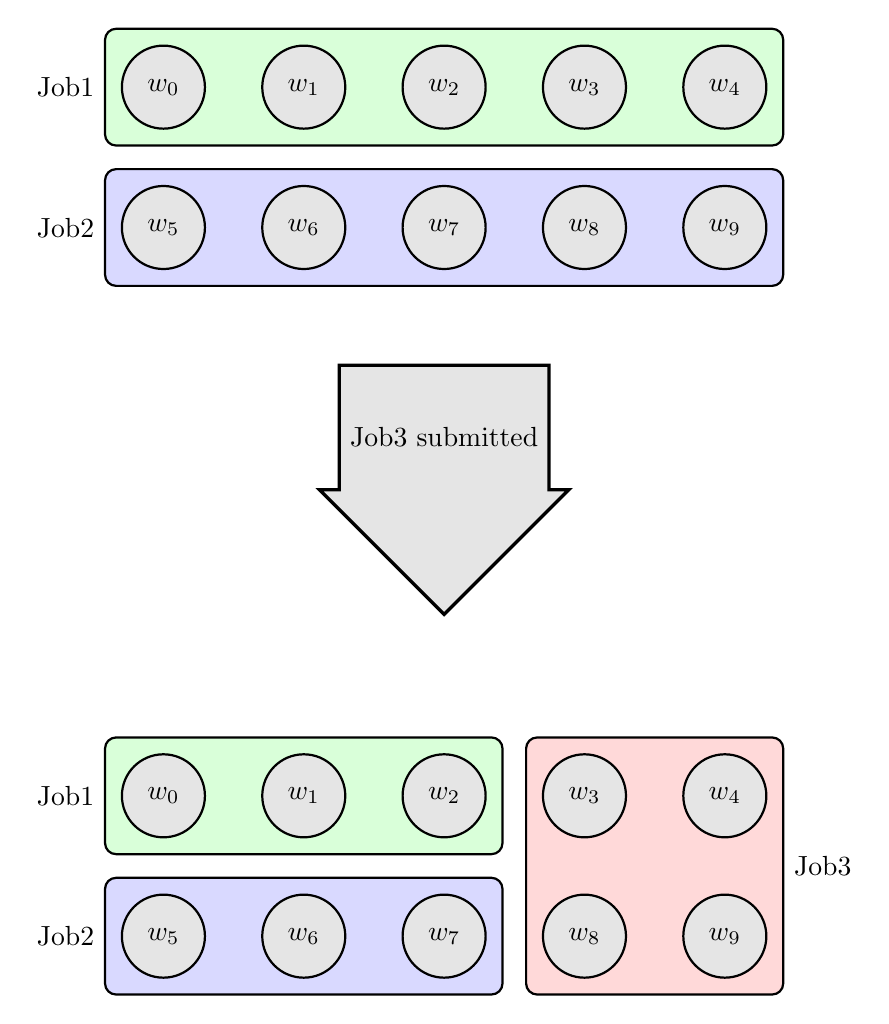
\begin{tikzpicture}
  % Workers on allocation 1
  \matrix (wmtrx1)[worker-matrix]{
	\node(w0){$w_0$};&	\node(w1){$w_1$};&	\node(w2){$w_2$};&	\node(w3){$w_3$};&	\node(w4){$w_4$};\\
	\node(w5){$w_5$};&	\node(w6){$w_6$};&	\node(w7){$w_7$};&	\node(w8){$w_8$};&	\node(w9){$w_9$};\\
  };
  \path (wmtrx1.south) +(0,-2cm) node[single arrow,draw=black,very thick,fill=black!10,minimum height=9em,shape border rotate=270]  {Job3 submitted};

  % Workers on allocation 2

  \matrix [yshift=-9cm](wmtrx2)[worker-matrix]{
	\node(w0_){$w_0$};&	\node(w1_){$w_1$};&	\node(w2_){$w_2$};&	\node(w3_){$w_3$};&	\node(w4_){$w_4$};\\
	\node(w5_){$w_5$};&	\node(w6_){$w_6$};&	\node(w7_){$w_7$};&	\node(w8_){$w_8$};&	\node(w9_){$w_9$};\\
  };

  \begin{pgfonlayer}{background}
    % Allocation 1
	\node [job-1, fit=(w0) (w4)] {};
	\node [job-2, fit=(w5) (w9)] {};

    % Allocation 2
	\node [job-1, fit=(w0_) (w2_)] {};
	\node [job-2, fit=(w5_) (w7_)] {};
	\node [job-3, fit=(w3_) (w9_)] {};
  \end{pgfonlayer}
\end{tikzpicture}

  \caption{Job allocation adjustment}
  \label{fig:allocation-adjustment}
\end{figure}
